\documentclass{article}

% Compiles on Overleaf (pdflatex, latexmk) and with `latexmk -pdf main.tex`: TeX Live packages only, no shell-escape.
\usepackage{arxiv}

\usepackage[utf8]{inputenc}
\usepackage[T1]{fontenc}
\usepackage{lmodern}
\usepackage{microtype}
\usepackage{amsmath}
\usepackage{amssymb}
\usepackage{booktabs}
\usepackage{tabularx}
\usepackage{array}
\usepackage{graphicx}
\usepackage{xcolor}
\usepackage{enumitem}
\usepackage{tikz}
\usetikzlibrary{arrows.meta,decorations.pathreplacing}
\usepackage[round,authoryear]{natbib}
\usepackage{url}
\usepackage{hyperref}
\usepackage{doi}

% What is missing, in red in the PDF.
\newcommand{\TODO}[1]{\textcolor{red}{[\textbf{TODO:} #1]}}
% The planned content of a section that is not drafted yet, in grey in the PDF.
\newenvironment{outline}{\par\color{gray}\small\noindent\textit{Outline, not drafted yet:}\begin{itemize}[nosep,leftmargin=*]}{\end{itemize}\par}
% A name taken from the software: a command, a file, a field of the record.
\newcommand{\code}[1]{\texttt{#1}}

\graphicspath{{figures/}}

% Working title: see notes/open-decisions.md.
\title{neuroimagym: step-based environments as a common medium for people and artificial agents in neuroimaging experiments}

\author{\TODO{Authors, affiliations and corresponding author: see notes/open-decisions.md}}

\begin{document}
\maketitle

\begin{abstract}
Naturalistic neuroimaging increasingly asks participants to act rather than watch, and computational neuroscience increasingly compares brains with artificial agents trained on the same tasks.
Both need a task that people and models can play identically, and a record that places every event of a run on the time base of the brain recording.
We present neuroimagym, open-source software that runs environments with the Gymnasium interface, the standard of reinforcement learning, as tasks in fMRI, MEG, EEG and behavioural sessions.
Its framework treats every task as an environment advanced in steps, and records for each step the screen flip that presented it, which translates exactly between the environment's engine time and the participant's human time.
Real-time games step at a fixed rate and puzzles at each decision; classical paradigms, in a regime we are building, step at each flip their script requests, so that all of them share one record, one replay mechanism and one set of players.
Around this core, neuroimagym describes each acquisition setup once, in a rig file that other programs can read; it measures display, audio and trigger timing; it synchronises with scanners and MEG and EEG systems; it records every input device; and it converts its logs to BIDS.
\TODO{validation results and use cases, one sentence each, once Sections~\ref{sec:validation} and~\ref{sec:use-cases} are written.}
\end{abstract}

\section{Introduction}
\label{sec:introduction}

\begin{outline}
  \item Neuroimaging is moving from controlled stimuli to naturalistic ones~\citep{sonkusare2019naturalistic,nastase2020keepitreal}, and from watching to acting: video games give rich, closed-loop tasks in which what the participant sees depends on what they did~\citep{cross2021deep,tomov2023neural,harel2023controller,boyle2025cneuromod}.
  \item A closed-loop stimulus can only be analysed if it can be reconstructed: the run must be replayable, frame by frame, from what was recorded.
  \item Comparing brains with artificial agents needs the same task for both. Reinforcement learning already has a common medium, the environment~\citep{brockman2016gym,towers2024gymnasium}, used for games~\citep{bellemare2013ale,mnih2015dqn} and for neuroscience tasks~\citep{molanomazon2022neurogym}; human experiments are written as scripts for experiment libraries~\citep{peirce2019psychopy,pallier2026goxpyriment}, whose timing has been compared in detail~\citep{bridges2020timing}.
  \item The gap: an environment knows only steps, a script knows only wall time, and neither records the translation between the two; a model's step cannot be aligned with a participant's brain signal unless that translation is part of the data.
  \item Contributions: (1) a framework in which every task is an environment stepped in one of three regimes, with a record that maps engine time to human time (Section~\ref{sec:framework}); (2) software that implements it for 15 game backends, with one record format and bit-exact replay (Sections~\ref{sec:architecture} and~\ref{sec:logging}); (3) a description of the acquisition setup and measurements of its timing that make the record trustworthy (Section~\ref{sec:multimodal}); (4) people and artificial agents on the same environments, with the same seeds and the same record (Section~\ref{sec:players}).
\end{outline}

\section{Framework}
\label{sec:framework}

An experiment in neuroimagym is a sequence of environments, each advanced one step at a time, and a run records when each step became visible to the participant.
Everything else follows from that relation between steps and time: playing one task with people and with artificial agents, aligning behaviour with brain signals, and reconstructing a run after the fact.
This section defines the environment, the two time bases an experiment lives on, the three ways an environment can be stepped, and what a run records so that each step can be placed on both time bases.
The terms defined here (Table~\ref{tab:vocabulary}) are the ones the software and its documentation use.

\subsection{Environments}
\label{sec:environments}

We call an environment any task that follows the interface of Gymnasium~\citep{towers2024gymnasium}, the maintained successor of OpenAI Gym~\citep{brockman2016gym}.
An environment is created, then advanced by two calls: \code{reset} starts an episode from a seed and returns the first observation, and \code{step} applies an action and returns the next observation, a reward, whether the episode has ended, and a dictionary of diagnostic information.
The interface was designed for reinforcement learning, and much of that field's benchmarks implement it, from Atari games~\citep{bellemare2013ale} to first-person 3D games~\citep{kempka2016vizdoom}, open-ended survival worlds~\citep{hafner2022crafter} and procedurally generated dungeons~\citep{kuttler2020nethack,samvelyan2021minihack}.
Neuroscience tasks have been written in the same form to train artificial networks on them~\citep{molanomazon2022neurogym}.
An environment is therefore a task that artificial agents can already play.

For an experiment with people, four properties of an environment matter.
First, the observation that counts is the rendered frame: the image, and the sound if there is any, that a person perceives.
Second, the environment is deterministic given its seed and its sequence of actions, so that any episode can be reconstructed exactly.
Third, the meaning of each action is declared, so that the mapping from a person's input devices to actions can be written down and checked.
Fourth, an environment that has a clock of its own declares its native rate, the number of steps per second at which it runs at its intended speed: an emulated home console runs at 60 frames per second, the Doom engine at 35 tics per second.

Nothing else is asked of an environment, and in particular it knows nothing about the experiment: it has no notion of a scanner, a participant, a trigger or a session.
All of that belongs to the layer that presents the environment to a person (Section~\ref{sec:architecture}), which keeps the environment identical for every player, human or artificial.
A game that ships no such environment is given a thin one, which adds the interface and nothing else.

\subsection{Engine time and human time}
\label{sec:time}

An experiment lives on two time bases.
Engine time is counted in steps: the state of an environment changes only when it is stepped, and nothing happens between two steps.
We write $k = 0, 1, 2, \dots$ for the steps of an environment.
When the environment has a native rate $r$, engine time can also be written in engine seconds, $k / r$.
Human time is the time of the participant and of the acquisition: seconds on one monotonic, high-resolution clock that every process of a run shares, with its origin at the start of the acquisition.
That origin is the scanner's trigger in fMRI, the start code sent to the recording in MEG and EEG, and the experimenter's start key when no acquisition device is involved.

The bridge between the two time bases is the screen flip.
The result of a step reaches the participant when the frame it produced is presented, and a display presents a new frame only at a vertical blank, once per refresh period~$T$ (16.7~ms at 60~Hz).
For every step, a run records $t_k$, the human time at which the flip that first presented the frame of step~$k$ completed.
Light reaches the eye a fixed delay later, at $t_k + \delta$, where $\delta$, the display's flip-to-photon latency, is measured once per rig with a photodiode (Section~\ref{sec:multimodal}).
Responses are stamped on the same clock, at the moment the run reads them, which is at most one refresh period after they happened; where the operating system provides it, each response also carries the input device's own timestamp.

Given the times $t_0 < t_1 < \dots$, any instant $t$ of human time maps to the step on screen,
\begin{equation}
  k(t) = \max\{\, k : t_k \le t \,\},
  \label{eq:step-on-screen}
\end{equation}
and any step maps to its onset, $t_k + \delta$.
This mapping is not a model of the task but a record of the run, exact up to the measured latencies.
When an environment has a native rate, the number of steps per second of human time divided by $r$ is the speed at which it was played.
A run reports that speed, so that a game slowed down for the scanner is never mistaken for one played at its intended pace.

Because flips happen only at vertical blanks, every step is shown for a whole number of refresh periods: $t_{k+1} - t_k = n_k T$, with $n_k \ge 1$, in a run that drops no frame.
The refresh period is thus the quantum of human time in any experiment shown on a screen, whatever the task: a fixation cross of 500~ms is 30 refreshes at 60~Hz, and a game frame at 60~Hz is one.
Classical paradigms are bound by this grid as much as games are: a stimulus cannot appear between two refreshes, and a response cannot answer a stimulus that is not yet on the screen.
This is what lets them be treated as environments too.

\subsection{Three stepping regimes}
\label{sec:regimes}

Environments differ in what decides when the next step happens.
We distinguish three stepping regimes (Table~\ref{tab:regimes}, Figure~\ref{fig:regimes}).

\begin{table}[t]
  \centering
  \small
  \caption{The three stepping regimes. $T$ is the display's refresh period; $n$ is a whole number of refresh periods.}
  \label{tab:regimes}
  \begin{tabularx}{\textwidth}{@{}l>{\raggedright\arraybackslash}X>{\raggedright\arraybackslash}X>{\raggedright\arraybackslash}X>{\raggedright\arraybackslash}p{2.2cm}@{}}
    \toprule
    Regime & The next step happens & Action & Examples & Status \\
    \midrule
    Fixed-rate & every $n$ refresh periods, at $f = 1/(nT)$ steps per second & the controls held at the step & arcade, console, first-person, racing and browser games & implemented \\
    Turn-based & at the first flip after a decision & the decision & sliding-block, rule-rewriting and grid-world puzzles & implemented \\
    Flip-locked & at each flip the task's script requests & a response and its reaction time, where the script waits for one & tasks written for PsychoPy or goxpyriment & planned; prototyped \\
    \bottomrule
  \end{tabularx}
\end{table}

\paragraph{Fixed-rate stepping.}
The environment advances one step every $n$ refresh periods, at a rate $f = 1/(nT)$ chosen to divide the refresh rate, whether or not the participant acts.
At each step, the action is read from the controls held at that moment, and holding nothing is an action like any other.
This is how real-time games are played: arcade, console, first-person, racing and browser games.
Engine time and human time then advance together, in the ratio $f/r$.
When the computer falls behind, the next step is scheduled from the late flip rather than from the missed one: the run never bursts through several steps to catch up, and it records the stall.

\paragraph{Turn-based stepping.}
The environment advances one step per decision, that is, per press of a control bound to an action.
Between two decisions, engine time stands still while human time flows: the interval from $t_k$ to $t_{k+1}$ is the time the participant took to decide, and it is part of the data rather than a pause in it.
Puzzles are played this way: sliding-block puzzles, rule-rewriting puzzles, grid worlds.
Some environments contain stretches in which they accept no decision, such as an avatar asleep until its energy is restored.
There, the environment says which action to apply, and the run steps it at a fixed rate, showing and recording every step, so that nothing is skipped and nothing is hidden.

\paragraph{Flip-locked stepping (planned).}
Classical neuroimaging tasks are written as scripts for an experiment library, such as PsychoPy~\citep{peirce2019psychopy} or goxpyriment~\citep{pallier2026goxpyriment}.
A script draws a screen, requests a flip, and waits, for a duration or for a response, before it draws the next one.
Each flip the script requests can be taken as one step.
The step's observation is the frame flipped; its duration is whatever the script waits until its next flip, a whole number of refresh periods; and its action, where the script waits for a response, is that response together with its reaction time, measured from the flip.
The script's own clock is the engine clock.
With a participant, it is the real clock, so that engine time and human time coincide on the refresh grid.
With an artificial agent, a virtual clock takes its place: a wait advances the clock without sleeping, a flip rounds the clock up to the next refresh, and a response arrives at the time its reaction time places it.
Run this way, an unmodified script becomes an environment like the games, with the same record, the same replay and the same players.
This regime is a design that the software does not implement yet.
A prototype ran an unmodified PsychoPy card-sorting script flip by flip on a virtual clock, with two independent implementations of the clock and of the responses, and both wrote the same results file \TODO{report the prototype and its measurements in Section~\ref{sec:use-cases}}.

All three regimes produce the same object: a sequence of steps, each shown for a whole number of refresh periods, each stamped in human time, each with the action that produced the next.
They differ only in what triggers the next step: a fixed schedule, the participant, or the task's script.
A run already chains phases of different kinds, such as a fixation, instructions, a turn-based puzzle and a real-time game, and records them in one format; the flip-locked regime adds classical tasks to the same chain.

\begin{figure}[t]
  \centering
  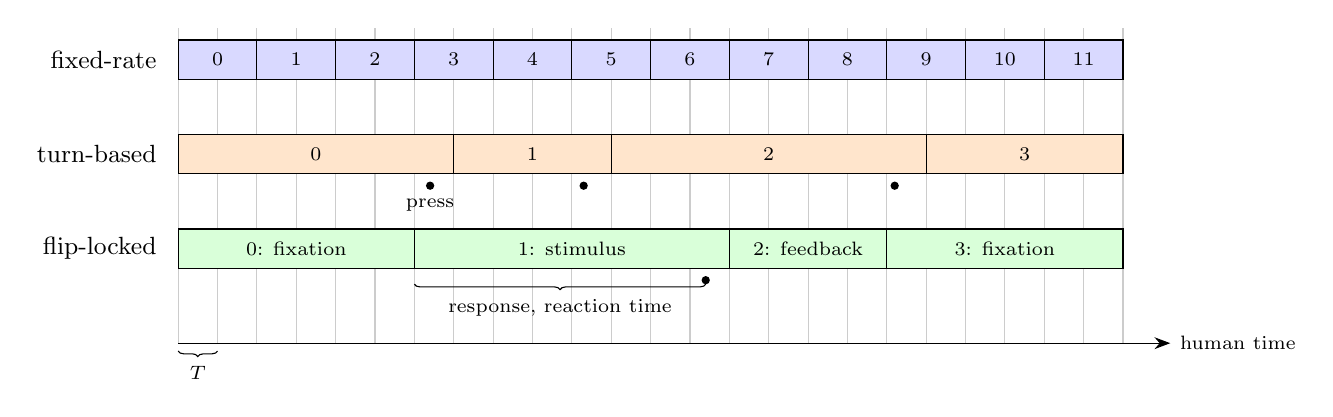
\begin{tikzpicture}[x=0.5cm,y=1cm,font=\scriptsize]
    % The refresh grid: one vertical line per vertical blank.
    \foreach \i in {0,...,24} {\draw[gray!40] (\i,-0.6) -- (\i,3.4);}
    \draw[-{Stealth[length=2mm]}] (0,-0.6) -- (25.2,-0.6) node[right] {human time};
    \draw[decorate,decoration={brace,mirror,amplitude=2pt}] (0,-0.7) -- (1,-0.7) node[midway,below=2pt] {$T$};
    % Fixed-rate: one step every two refresh periods.
    \node[anchor=east,font=\small] at (-0.3,3.0) {fixed-rate};
    \foreach \k in {0,...,11} {
      \draw[fill=blue!15] ({2*\k},2.75) rectangle ({2*\k+2},3.25);
      \node at ({2*\k+1},3.0) {\k};
    }
    % Turn-based: one step per decision, shown at the first flip after the press.
    \node[anchor=east,font=\small] at (-0.3,1.8) {turn-based};
    \foreach \a/\b/\k in {0/7/0,7/11/1,11/19/2,19/24/3} {
      \draw[fill=orange!20] (\a,1.55) rectangle (\b,2.05);
      \node at ({(\a+\b)/2},1.8) {\k};
    }
    \foreach \p in {6.4,10.3,18.2} {\fill (\p,1.4) circle (1.5pt);}
    \node[anchor=north] at (6.4,1.35) {press};
    % Flip-locked: one step per flip the script requests, as long as the script waits.
    \node[anchor=east,font=\small] at (-0.3,0.6) {flip-locked};
    \foreach \a/\b/\k/\what in {0/6/0/fixation,6/14/1/stimulus,14/18/2/feedback,18/24/3/fixation} {
      \draw[fill=green!15] (\a,0.35) rectangle (\b,0.85);
      \node at ({(\a+\b)/2},0.6) {\k: \what};
    }
    \fill (13.4,0.2) circle (1.5pt);
    \draw[decorate,decoration={brace,mirror,amplitude=2pt}] (6,0.15) -- (13.4,0.15) node[midway,below=2pt] {response, reaction time};
  \end{tikzpicture}
  \caption{The three stepping regimes on the display's refresh grid (one vertical line per refresh period~$T$). Each box is one step, from the flip that first shows it to the next flip; the numbers are step indices. Fixed-rate: a step every two refresh periods, whatever the participant does. Turn-based: a step at the first flip after each press (dots). Flip-locked: a step at each flip a task's script requests, for as long as the script waits; the response, with its reaction time measured from the stimulus' flip, is that step's action.}
  \label{fig:regimes}
\end{figure}

\subsection{Decision points and actions}
\label{sec:actions}

A decision point is a step whose transition depends on an action.
In fixed-rate stepping, every step is one.
In turn-based stepping, every step is one, and nothing happens between them.
In flip-locked stepping, only the flips after which the script waits for a response are, and the script itself says where they are, by waiting.
For an artificial agent, the decision points are where it is asked to act; between them, the environment runs on its own.

Actions are written in the environment's own action space: an index into a set of discrete actions, a set of buttons, a vector of continuous values, or, for a scripted task, a response with its reaction time.
A person's input devices are mapped onto that space by an explicit table, from named controls (a key, a button, a direction of a stick, an axis) to actions, written in the definition of the task.
There is no default mapping, so that the table is the documented truth of what each control did.
The keys with which the experimenter starts and stops a run are reserved and can never be bound to an action.

Inputs are registered between flips.
The run reads every event that arrived since the previous flip, stamps it when read, and combines the controls held and the controls pressed into the action of the next step, so that a tap shorter than a step still counts.
When the input devices are also recorded by the operating system alongside the run (Section~\ref{sec:multimodal}), each event carries the system's own timestamp on the same clock, which removes the uncertainty of the reading time.

\subsection{One environment, two kinds of player}
\label{sec:players}

The same environment is played by people and by artificial agents, and the framework makes explicit what the two share and what they do not.
They share the environment's code and version; the seeds, and therefore the episodes; the action space; the observation, which is the frame a participant sees; and the format of the record.
They differ in how actions are produced and in how human time passes.
A participant plays on the real clock: the display paces the steps, and actions come from input devices through the rig (Section~\ref{sec:architecture}).
An artificial agent plays on a virtual clock: steps advance as fast as the policy computes, and the policy chooses an action at each decision point.
Engine time is the same for both; only its mapping to human time differs, and for an agent that mapping is either absent, in fixed-rate and turn-based environments, or simulated, in flip-locked environments, where the reaction time is part of the action.

Two constraints keep the comparison meaningful.
First, a policy sees only what a participant sees: the frames and the instructions.
The environment's internal state is recorded for analysis and never handed to the policy, since a policy given the engine's state no longer plays the game the person played.
Second, the rules of a task live in the environment and nowhere else.
The layer that presents an environment to a person may add an experimental frame around it (fixations, instructions, a pause menu, a status line that shows what the environment reports), but never a rule, an affordance or a score of its own; if it did, people and models would be playing different tasks.

Under these constraints, a model can be scored on exactly the episodes a participant played, by playing with the same seeds.
It can also be given the participant's own observations and actions, step by step, to read out its internal states, which yields regressors for the neuroimaging data on the participant's engine time, mapped to human time by the run's record.

\subsection{What a run records}
\label{sec:record}

Each of these properties is only as good as its record.
For every step, a run writes its index, the action applied, the human time of the flip that showed it, the variables the environment reports (a score, a position, a game's internal state), and, at a chosen interval, a savestate from which the environment can be restored exactly.
For every input event and every code sent to an acquisition device, it writes the human time at which it happened.
For the run as a whole, it writes the full configuration (the definition of the task, the rig, the software versions and the machine) and the seeds.

From this record, one can derive the onset and duration of every step and event, every reaction time, an events table in the Brain Imaging Data Structure~\citep{gorgolewski2016bids}, and, after replay, any variable of the environment at any step.
Replay is part of the framework rather than a convenience: a run is reconstructed bit for bit in a separate process, from its seeds and actions or from its savestates, and the software tests this for every backend its test suite plays (Section~\ref{sec:validation}).
A record is never overwritten: a run played again is written next to the first one, with the same seeds.

The units of the record follow from the framework.
A run is one process that plays one curriculum, the file that defines a sequence of phases (fixations, messages, surveys and environments), and writes one folder.
A block is one environment phase as played within a run.
An episode goes from a reset to the end of the environment's task.
A session is the ordered list of runs a participant does in one visit.

\subsection{Vocabulary}
\label{sec:vocabulary}

Table~\ref{tab:vocabulary} gathers the terms defined in this section.
The software's documentation uses the same words, with the same meanings.

\begin{table}[t]
  \centering
  \small
  \caption{The vocabulary of the framework, shared with the software's documentation. Where the software uses another name for the same thing, it is given in brackets.}
  \label{tab:vocabulary}
  \begin{tabularx}{\textwidth}{@{}l>{\raggedright\arraybackslash}X@{}}
    \toprule
    Term & Meaning \\
    \midrule
    environment & A task with the Gymnasium interface: reset from a seed, step with an action. Its observation, for a person, is the rendered frame. \\
    backend & The integration of one engine or runtime that produces environments: an emulator, a game engine, a browser, an experiment library. \\
    step & One transition of an environment; the unit of engine time. \\
    engine time & Time counted in steps, or in engine seconds when the environment has a native rate. \\
    human time & Seconds on the run's clock, from the start of the acquisition [\code{run\_time}]. \\
    flip & The presentation of a frame at a vertical blank; it ties a step to human time. \\
    refresh period & The interval between two vertical blanks; the quantum of human time on a screen. \\
    stepping regime & What triggers the next step: a fixed schedule (fixed-rate), a decision (turn-based), or the task's script (flip-locked). \\
    action & What an environment receives at a step: a discrete choice, a set of buttons, continuous values, or a response with its reaction time. \\
    control & A named key, button, stick direction or axis of an input device, mapped to actions by the curriculum. \\
    decision point & A step whose transition depends on an action. \\
    episode & From a reset to the end of the environment's task. \\
    phase & One entry of a curriculum: a fixation, a message, a survey, or an environment [\code{game}]. \\
    block & An environment phase as played in a run. \\
    curriculum & The file a run plays: an ordered list of phases, the same for every participant and every rig. \\
    run & One curriculum played once by one participant: one command, one process, one data folder. \\
    session & The runs a participant does in one visit, in order, written as a session script. \\
    rig & One acquisition setup (computer, screen, input devices, trigger line), described once in a rig file. \\
    participant, agent & A person, or an artificial policy, playing an environment. \\
    real clock, virtual clock & Wall time, for participants; a clock that advances only when the task says so, for agents, tests and replay. \\
    savestate & A snapshot from which an environment is restored exactly. \\
    replay & Rebuilding a run's frames and states from its seeds and actions, or from its savestates. \\
    \bottomrule
  \end{tabularx}
\end{table}

\section{Architecture}
\label{sec:architecture}

\begin{outline}
  \item Three layers per game, each in its own place and each optional until needed: the game's own code, pinned (a package or a checked-out repository); a thin environment package when the game ships no Gymnasium environment; and one adapter per backend, which builds the environment, maps controls to actions, renders frames and sound, and reports what to record.
  \item The run never knows the engine: it calls only the adapter; game engines are imported only by adapters; the layers import only downwards, and a contract checked in continuous integration enforces it.
  \item Three kinds of settings, kept apart because they are shared differently: the curriculum (what is played, the same for every participant and site), the rig (how this setup plays every run), and the run's own numbers (participant, session, run, duration). Neither file names the other; what needs both is decided when the run starts.
  \item One run is one process, one command and one data folder; a session is a plain shell script with one line per run, written by hand or by a tool, and managed, if wanted, by a session launcher \TODO{name the compatible launchers}.
  \item Tools that can run on their own stay outside the run: making and measuring a rig, calibrating a controller, recording the session's input devices, converting logs. The run only reads what they filed, at start-up.
  \item Checks at the desk: every problem that can be found before the participant's screen opens stops the run there, with the fix in the message; a default that changes what is recorded is printed and recorded, never silent.
  \item Install only what is needed: each backend is an optional extra, imported only when a curriculum names it.
  \item Table: the 15 backends, their action spaces, how their savestates work, and their platforms \TODO{generate from the software's backend list}.
\end{outline}

\section{Logging and reproducibility}
\label{sec:logging}

\begin{outline}
  \item The record of a run (Section~\ref{sec:record}) in files: a manifest with the full configuration, the versions and the machine; the run's log of everything read, shown, sent and printed; one log per block with every step, its frames and its sound.
  \item Written by a separate process and flushed every second, so that a crash loses at most the last second; nothing is ever overwritten, and a run played again goes to a new folder with the same seeds.
  \item Savestates: the engine's own snapshot where it has one; otherwise the seed and the actions since the reset, restored by replaying them, which makes any deterministic environment restorable.
  \item Bit-exact replay in a second process, tested for every backend the suite plays \TODO{number of backends and frames compared}.
  \item Provenance: every manifest names the code version (and whether it had uncommitted changes), the libraries and the machine.
  \item Resuming: a curriculum belongs to the participant and a run to the acquisition; a run can stop anywhere, and a later run continues from the recorded state.
  \item From logs to BIDS: events tables, a participants table, and readable timelines of each run, joined with the session's recording of the input devices.
\end{outline}

\section{Multimodal integration}
\label{sec:multimodal}

\begin{outline}
  \item The rig file: one description of an acquisition setup (screen and its geometry, input devices, sound, trigger line, photodiode, fixations, data folder), in the repository, reviewed with the code, copied into every run's record, and read by other experiment programs as well \TODO{a versioned schema for those programs}.
  \item Starting a run: wait for the scanner's trigger, send a start code to a MEG or EEG recording, or start at once; the origin of human time (Section~\ref{sec:time}).
  \item Codes sent during a run: bits for each frame and for the run's lifecycle, or for the participant's responses, over the lab's line (Lab Streaming Layer, serial, parallel, USB data-acquisition boxes) \TODO{cite LSL once its reference is verified}.
  \item The display: a fixed canvas scaled to any monitor; vertical synchronisation measured, not assumed; every flip stamped; a photodiode patch that alternates with each frame.
  \item Sound: the game's own audio, each chunk placed a measured delay after its frame's flip.
  \item Input devices: keyboards, gamepads and MRI- and MEG-compatible controllers under one vocabulary of named controls~\citep{harel2023controller}; per-machine calibration of analogue sticks.
  \item A recording of every input device the operating system sees, for the whole session, with the system's own timestamps on the run's clock, plus focus changes and machine stalls.
  \item Measuring the rig: display, frame pacing, triggers, controls, photodiode and audio, short before each session and long once per setup, with reports pooled across sites.
  \item Eye tracking \TODO{the current integration and its plan}.
\end{outline}

\section{Validation}
\label{sec:validation}

\begin{outline}
  \item Frame pacing and vertical synchronisation on the acquisition rigs: distribution of flip intervals, dropped frames \TODO{numbers from the long rig measurements}.
  \item Flip-to-photon and audio latencies per rig, measured with a photodiode and a microphone \TODO{numbers}.
  \item Input latency: time of reading versus the operating system's timestamps \TODO{numbers from a session recording}.
  \item Replay: every backend the test suite plays is replayed bit for bit in a second process \TODO{backends, frames, mismatches}.
  \item Continuous integration: every backend that a Linux runner can play, every curriculum validated against its example rig.
\end{outline}

\section{Use cases}
\label{sec:use-cases}

\begin{outline}
  \item Games in fMRI and MEG sessions of a longitudinal study \TODO{sites, participants, sessions, games, hours}.
  \item Artificial agents on the participants' curricula: a random policy and a vision-language model playing the same environments, with the same record \TODO{results}.
  \item Classical tasks as environments: the flip-locked prototype on a card-sorting task \TODO{numbers from the prototype: flips, task time, computation time, results identical between two implementations}.
  \item Replaying a participant's run through a model to obtain step-by-step regressors \TODO{an example}.
\end{outline}

\section{Discussion}
\label{sec:discussion}

\begin{outline}
  \item What the framework buys: one record and one replay for any screen-based task, and a translation between engine time and human time that is measured rather than assumed.
  \item Limits: the refresh grid bounds the precision of every onset; consumer hardware and operating systems differ in timing; the flip-locked regime is not yet run with participants; some backends need a real display, which complicates headless use.
  \item Related software: experiment libraries~\citep{peirce2019psychopy,pallier2026goxpyriment}, task collections for artificial networks~\citep{molanomazon2022neurogym}, game benchmarks~\citep{bellemare2013ale,kempka2016vizdoom,hafner2022crafter,samvelyan2021minihack,tomilin2023coom,cloos2024babaisai}; what neuroimagym adds to each.
  \item Future work: the flip-locked regime for classical tasks; a schema of the rig file for the other programs that read it; more acquisition setups.
\end{outline}

\section*{Code availability}

\TODO{Repository URL after the rename, the release cited, and the licence (the repository has none yet).}

\section*{Acknowledgements}

\TODO{Funding and acknowledgements.}

\section*{Author contributions}

\TODO{Contributions.}

\section*{Competing interests}

\TODO{Competing interests.}


\bibliographystyle{plainnat}
\bibliography{references}

\end{document}
